\documentclass[12pt]{beamer}
\usepackage[utf8]{inputenc}
\usepackage[spanish]{babel}
\usepackage{amsmath}
\usepackage{amsfonts}
\usepackage{amssymb}
\usepackage{graphicx}
\usepackage{mathrsfs} 
\usepackage{outlines}
\usetheme{Goettingen}
%\usepackage{subfig,graphicx,showframe}
\setbeamertemplate{bibliography item}[text]
\DeclareMathOperator{\re}{Re}
\setbeamertemplate{footline}[frame number]
\begin{document}
	\author{Carlos Daniel Contreras Quiroz}
	\title{Desarrollo de un programa de lectura y análisis de películas radiocrómicas para verificación dosimétrica}
	%\subtitle{}
	\logo{
\includegraphics{images/logo.png}}
	\institute{Universidad de los Andes}
	%\date{}
	%\subject{}
	%\setbeamercovered{transparent}
	%\setbeamertemplate{navigation symbols}{}
	\begin{frame}[plain]
	\maketitle
\end{frame}

\begin{frame}{Contenido}
\tableofcontents
\end{frame}

\section{Introducción}
\begin{frame}
\vfill
\centering
\begin{beamercolorbox}[sep=8pt,center,shadow=true,rounded=true]{title}
	\usebeamerfont{title}\insertsectionhead\par%
\end{beamercolorbox}
\vfill
\end{frame}

\subsection{Películas radiocrómicas}
\begin{frame}{Motivación}
En los procedimientos en radioterapia se requiere asegurar que las distribuciones de dosis planeadas correspondan con las ejecutadas realmente.  \\~\\

\begin{figure}
	\centering
	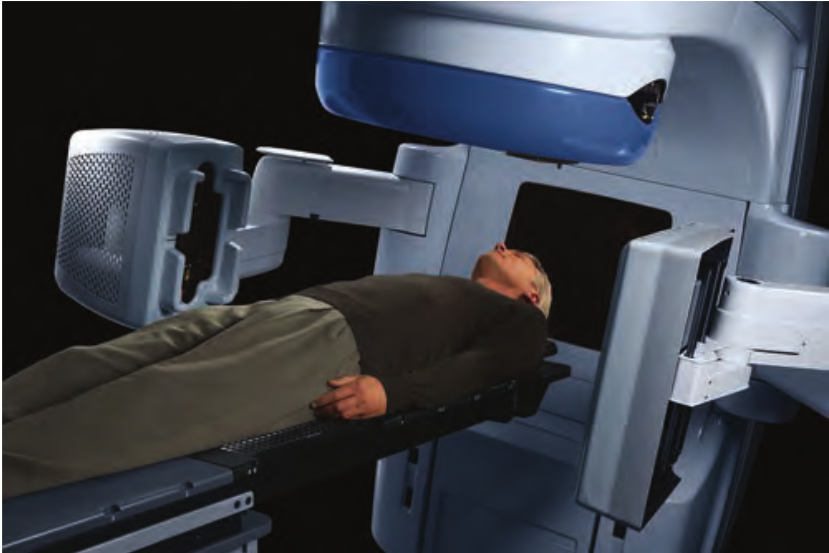
\includegraphics[width=0.7\linewidth]{images/paciente.png}
	\caption{Maquina Varian Trylogy \cite{khan2014the}}
\end{figure}

\end{frame}



\begin{frame}{Motivación}
Películas radiocrómicas
\begin{figure}[htp]% [H] is so declass\'e!
	\centering
	\begin{minipage}{0.45\textwidth}
		
\includegraphics[width=\textwidth]{images/fondoblancoLandscape-1.png}
		\caption{Película EBT2}
	\end{minipage}\hfill
	\begin{minipage}{0.45\textwidth}
		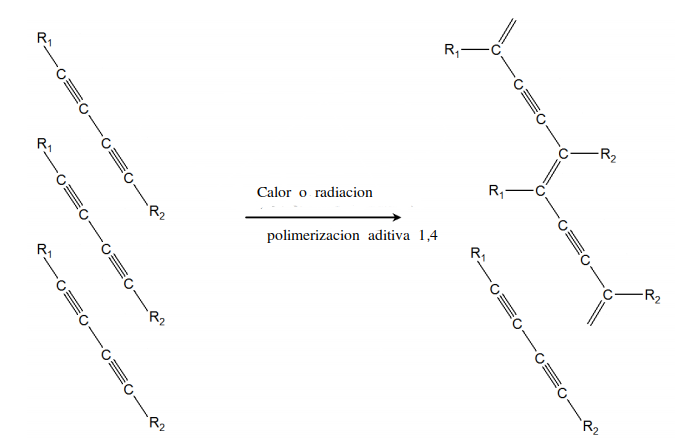
\includegraphics[width=\textwidth]{images/reaccion.png}
		\caption{Reacción de diacetileno\cite{Williams2011}}
	\end{minipage}\par
	\vskip\floatsep% normal separation between figures
	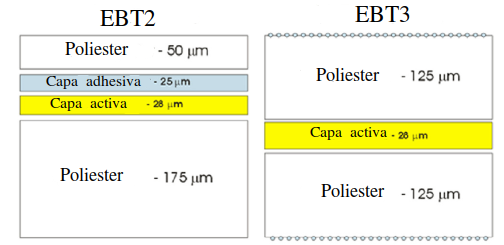
\includegraphics[width=0.45\textwidth]{images/estructuraEBT.png}
	\caption{Estructura de películas EBT\cite{Devic2016}}
\end{figure}
\end{frame}


\begin{frame}{Motivación}
	El uso de estas presenta varias ventajas
	\begin{itemize}
		\item Alta sensibilidad a la dosis(0.1 Gy-10Gy)
		\item Sin dependencia energética(50keV-10 MeV)
		\item Alta resolución espacial
		\item Practicas de usar
	\end{itemize}
\end{frame}

\begin{frame}{Uso de películas}
Para usarlas es necesario establecer un protocolo que correlacione cambios de color con dosis absorbida a traves de una calibración. Este debe tener en cuenta
\begin{itemize}
	\item Efectos de diversos parámetros(Temperatura, Orientación ...)
	\item Tipo de calibración y su utilidad
	\item Cuidados con la película
\end{itemize}
\end{frame}

\subsection{Objetivos}
\begin{frame}{Objetivos}
	\begin{outline}
		\1 Entender y aplicar el funcionamiento de películas radiocrómicas en verificación dosimétrica
		\2 Realizar calibraciones de dosis
		\2 Obtener mapas de dosis de un tratamiento a partir de una película
		\2 Realizar la comparación con el plan esperado
		\1 Desarrollar un software que permita su uso bajo diferentes modalidades para su uso en el CCC
	\end{outline}
\end{frame}

\section{Metodología}
\begin{frame}
	\vfill
	\centering
	\begin{beamercolorbox}[sep=8pt,center,shadow=true,rounded=true]{title}
		\usebeamerfont{title}\insertsectionhead\par%
	\end{beamercolorbox}
	\vfill
\end{frame}

\subsection{Adquisición de imágenes}

\begin{frame}{Montaje de irradiación}
\begin{figure}[htp]% [H] is so declass\'e!
	\centering
	\begin{minipage}{0.45\textwidth}
		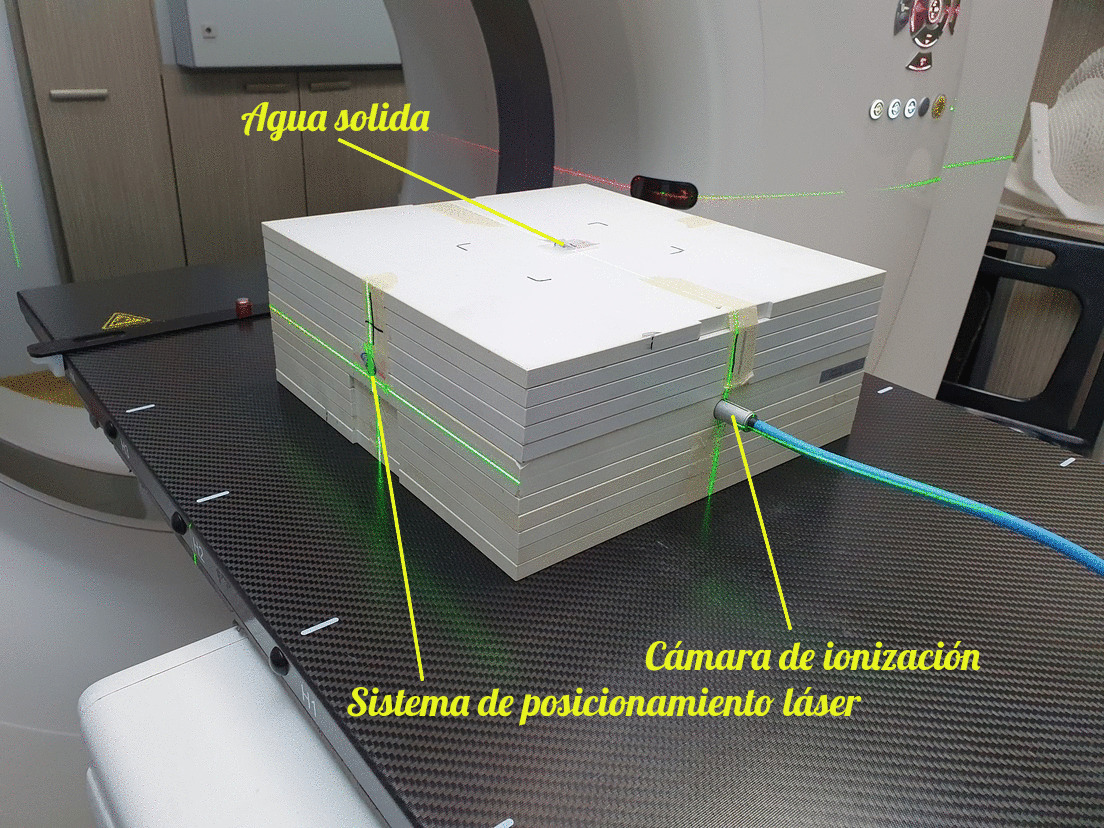
\includegraphics[width=\textwidth]{images/elctrometro.jpg}
	\end{minipage}\hfill
	\begin{minipage}{0.45\textwidth}
		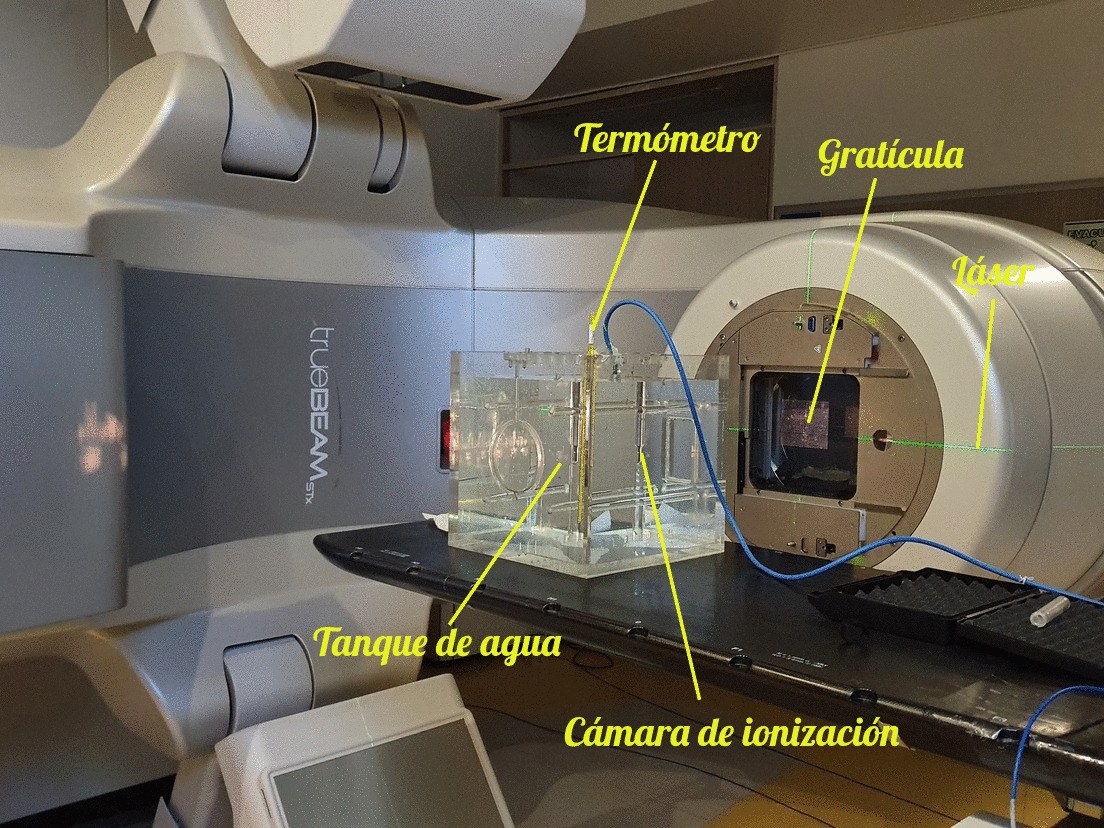
\includegraphics[width=\textwidth]{images/TRS398Editado2.jpg}
	\end{minipage}\par
	\vskip\floatsep% normal separation between figures
	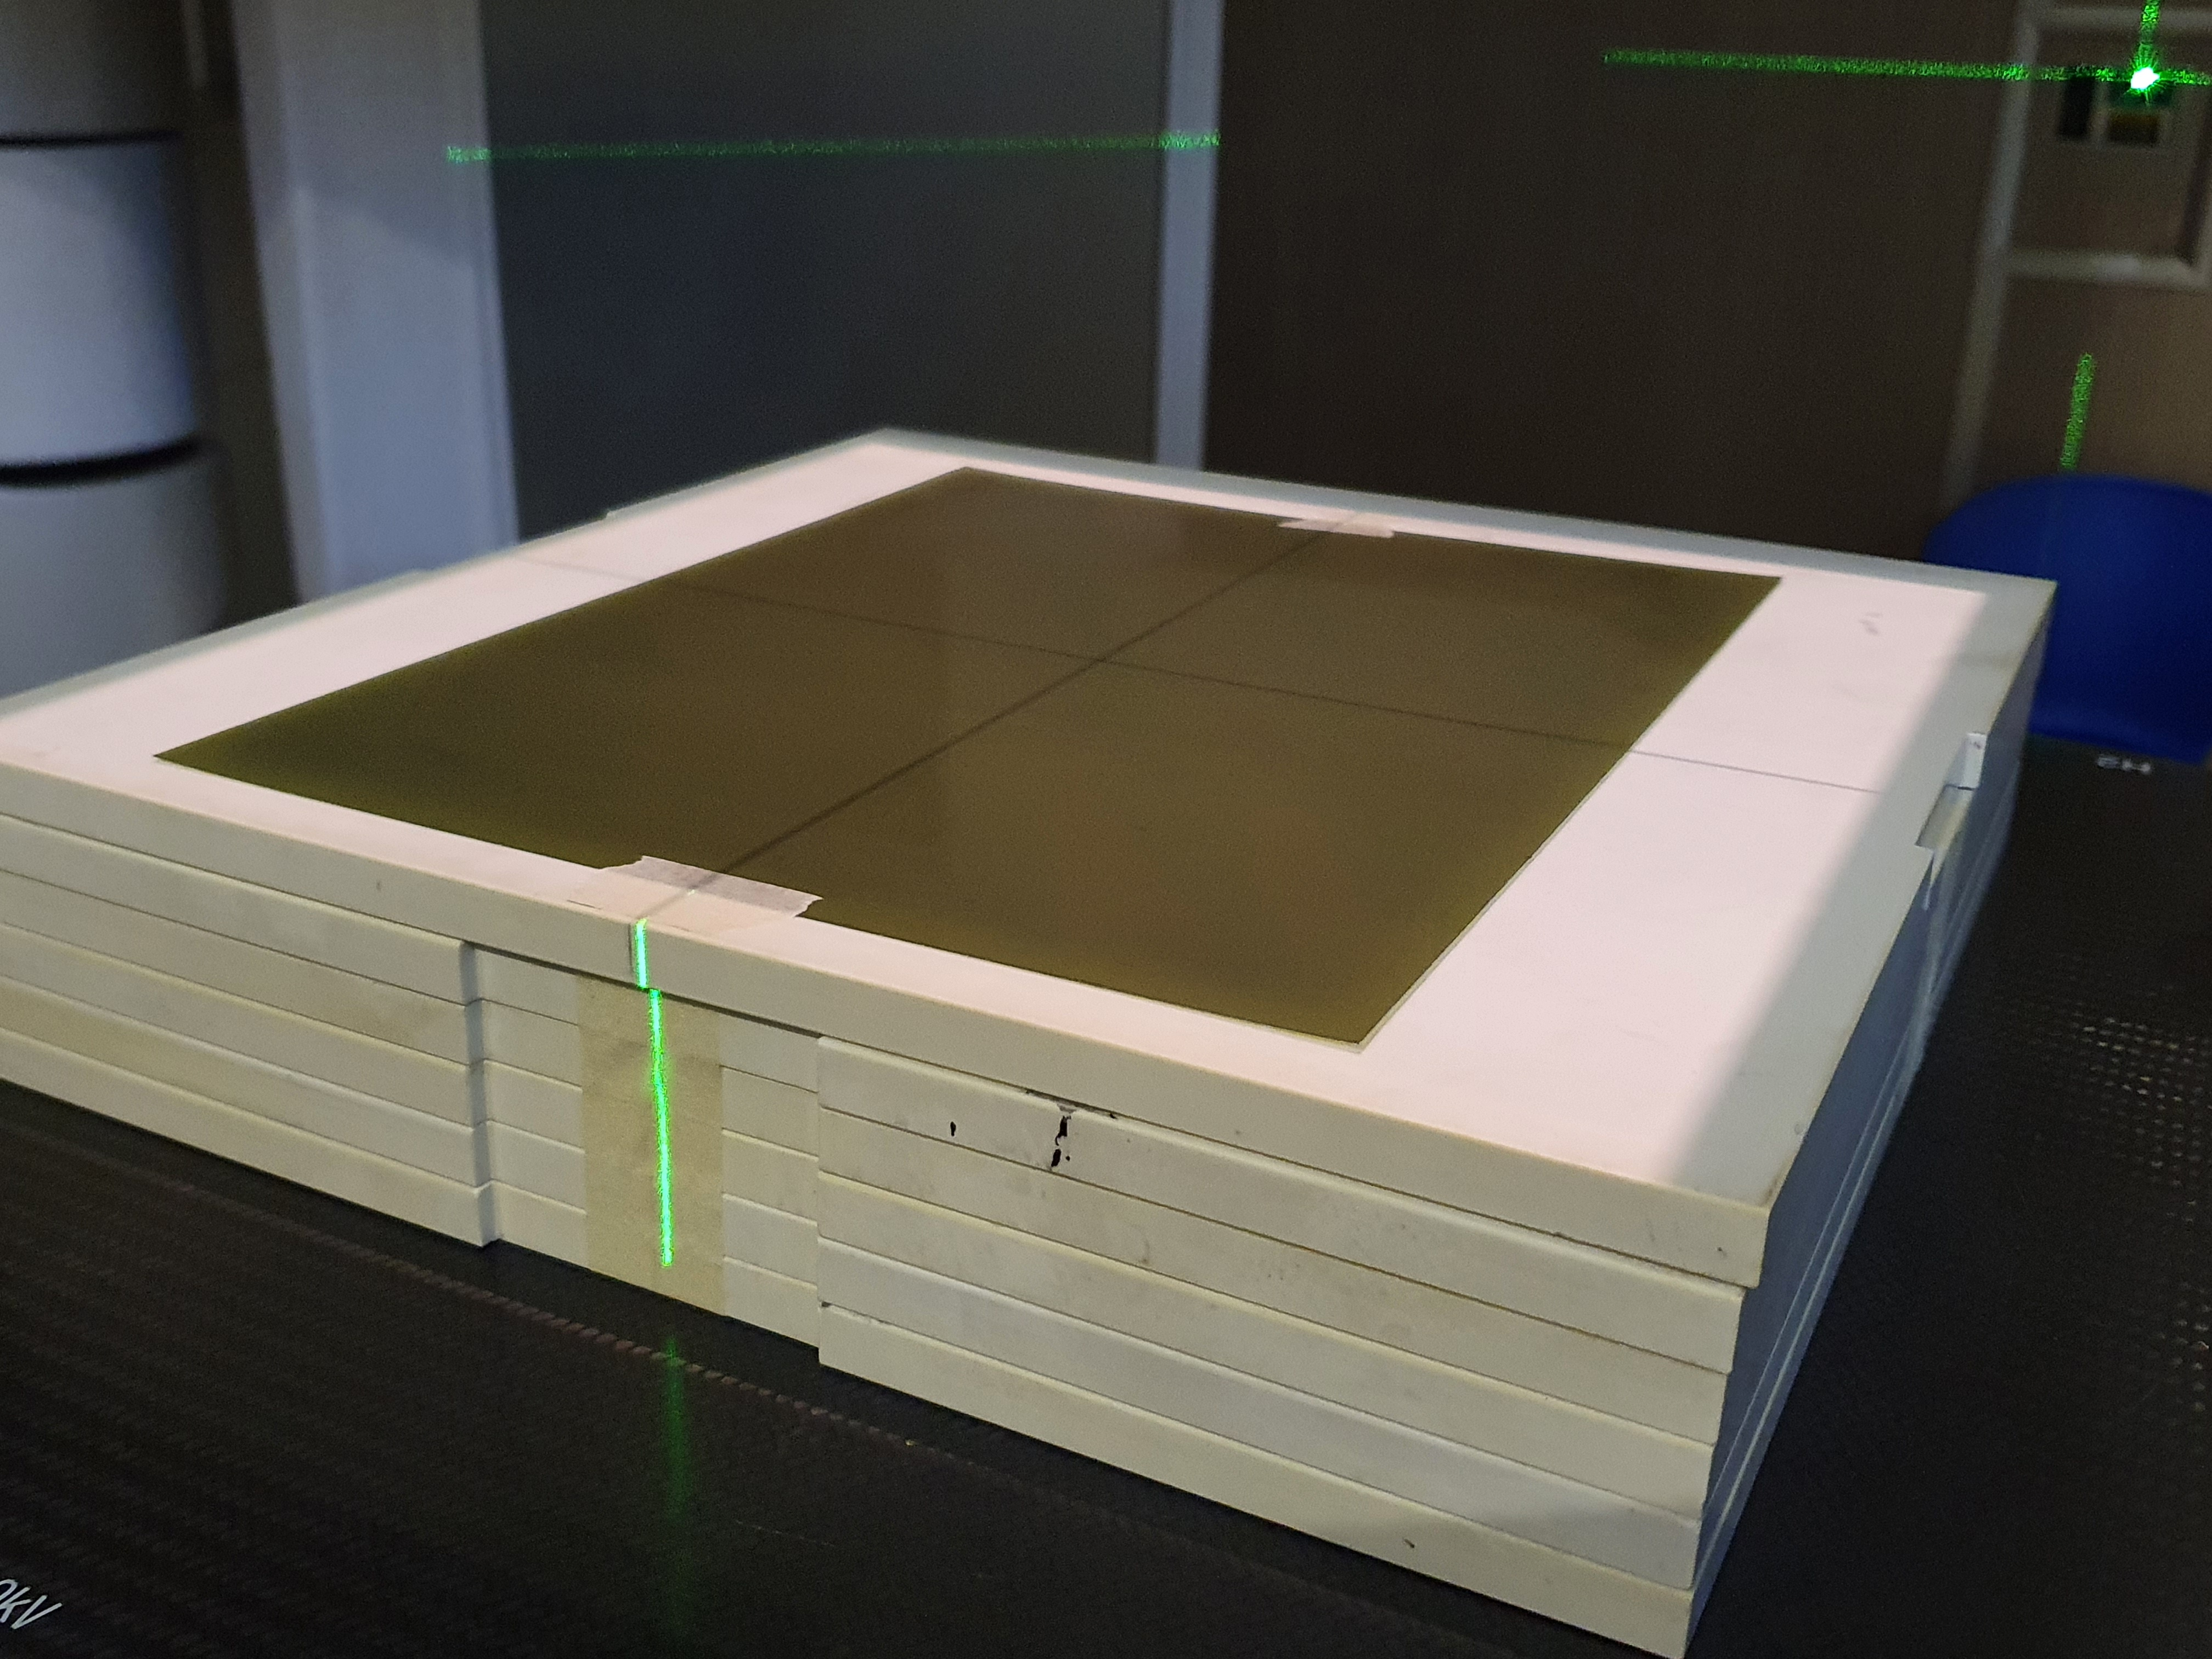
\includegraphics[width=0.45\textwidth]{images/20200826_215214.jpg}
\end{figure}
\end{frame}

\begin{frame}{Películas irradiadas}
\begin{figure}
	\centering
	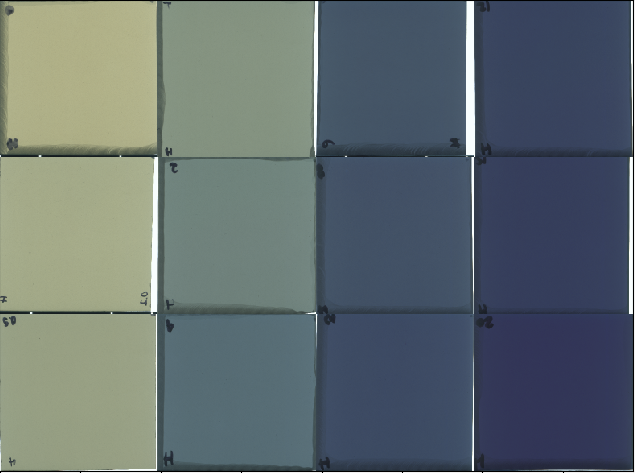
\includegraphics[width=0.7\linewidth]{images/peliculasIrradiadas.png}
	\caption{Películas irradiadas con dosis de 0 a 20 Gy}
\end{figure}

\end{frame}

\begin{frame}{Películas irradiadas}
\begin{figure}
	\centering
	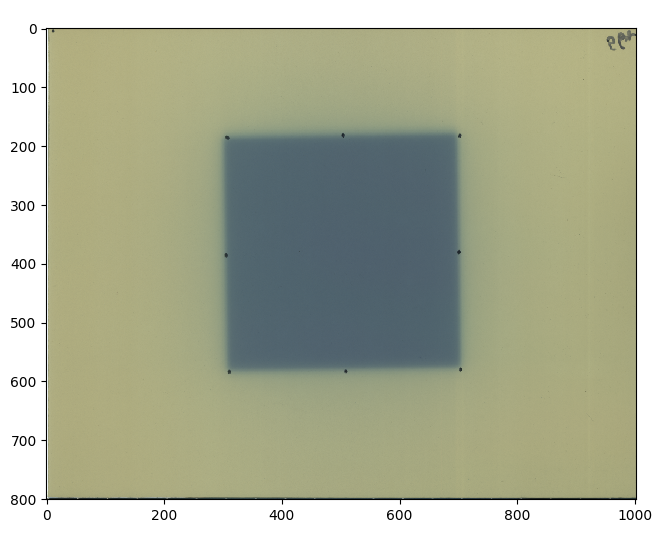
\includegraphics[width=0.7\linewidth]{images/peliculaCuadrado.png}
	\caption{Cuadrado irradiado con 5Gy}
\end{figure}
\end{frame}

\begin{frame}{Películas irradiadas}
\begin{figure}[htp]% [H] is so declass\'e!
	\centering
	\begin{minipage}{0.45\textwidth}
		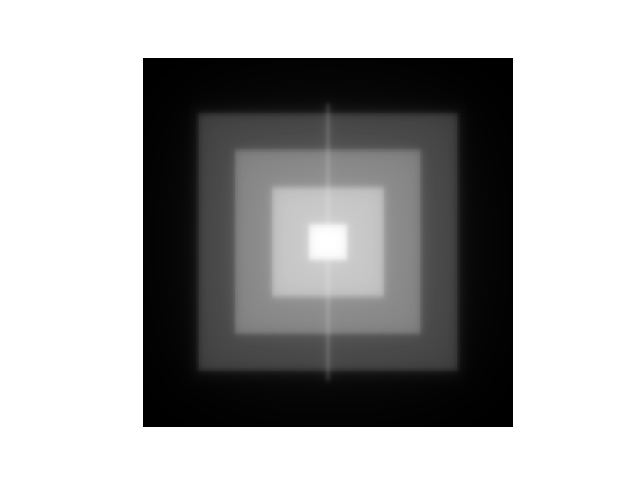
\includegraphics[width=\textwidth]{images/piramideTPS.png}
	\end{minipage}\hfill
	\begin{minipage}{0.45\textwidth}
		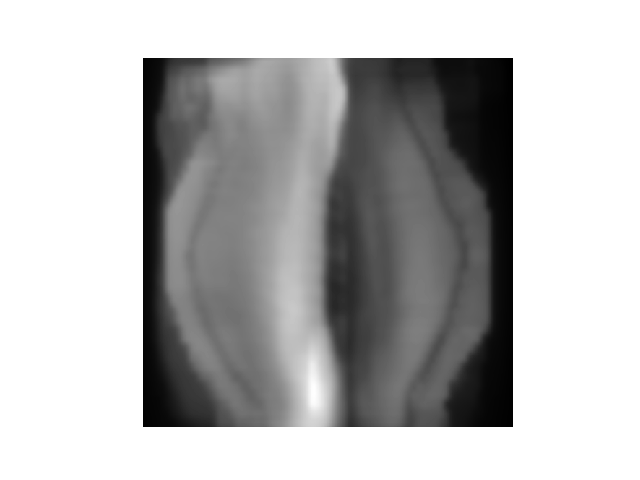
\includegraphics[width=\textwidth]{images/mamaTPS.png}
	\end{minipage}\par
	\begin{minipage}{0.45\textwidth}
	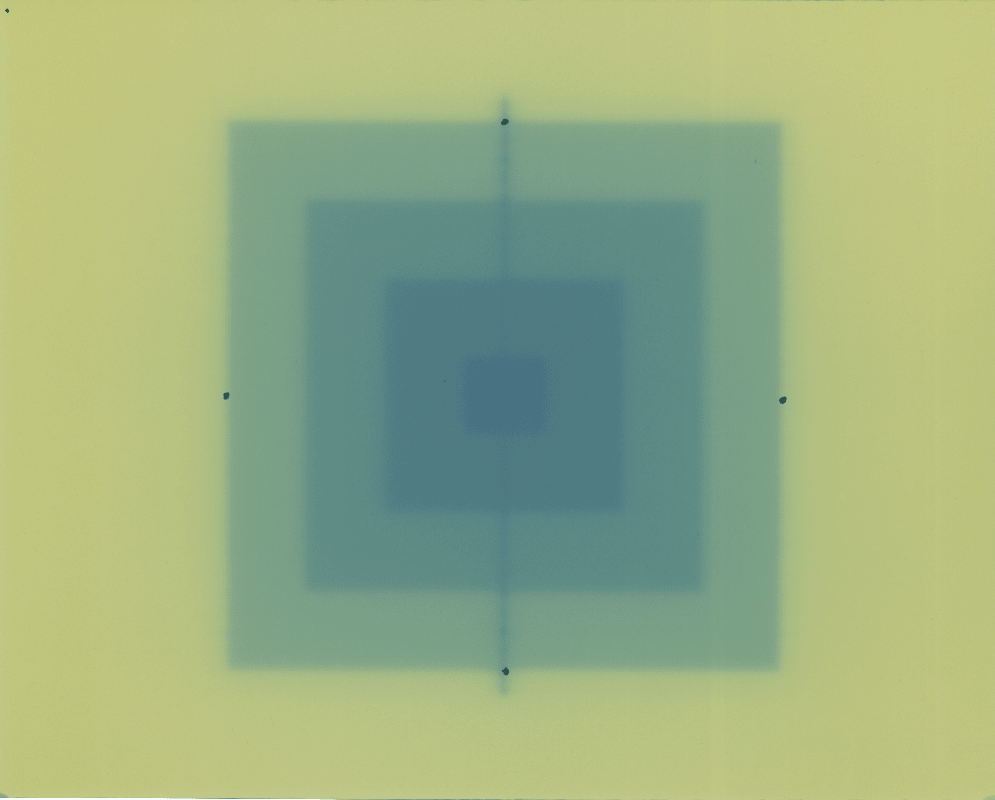
\includegraphics[width=\textwidth]{images/peliculaPiramide.png}
\end{minipage}\hfill
\begin{minipage}{0.45\textwidth}
	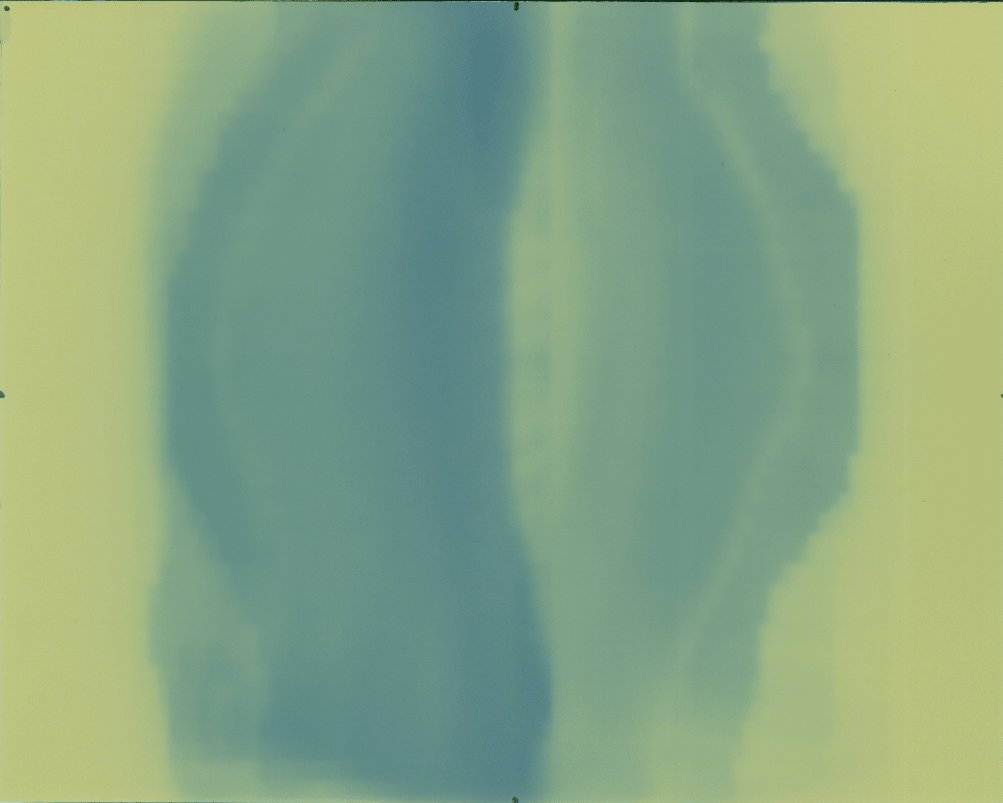
\includegraphics[width=\textwidth]{images/peliculaMama.png}
\end{minipage}
\caption{Mapas de dosis irradiados}
\end{figure}
\end{frame}


\begin{frame}{Digitalización}
Se digitalizaron las imágenes con un escáner  ScanMaker1000XL en modo transmisión.\\~\\

Se usó una resolución de 100 ppi con 16-bits por canal de color.\\~\\

Se probaron varios filtros sobre las imágenes, entre ellos el filtro de Wiener, el filtro de mediana y el filtro de promediado.\\~\\
\end{frame}

\subsection{Características del programa}

\begin{frame}{Programa}
Para realizar el análisis de manera eficiente se desarrollo un programa en Python que comprende la siguientes funcionalidades
\begin{itemize}
	\item Generación de curvas.
	\item Generación y adecuación de mapas de dosis.
	\item Comparación con planes de tratamiento.
	\item Herramientas varias.
\end{itemize}
\end{frame}

\section{Resultados}
\begin{frame}
\vfill
\centering
\begin{beamercolorbox}[sep=8pt,center,shadow=true,rounded=true]{title}
	\usebeamerfont{title}\insertsectionhead\par%
\end{beamercolorbox}
\vfill
\end{frame}

\subsection{Calibración}

\begin{frame}{Curvas de calibración}
\begin{figure}
	\centering
	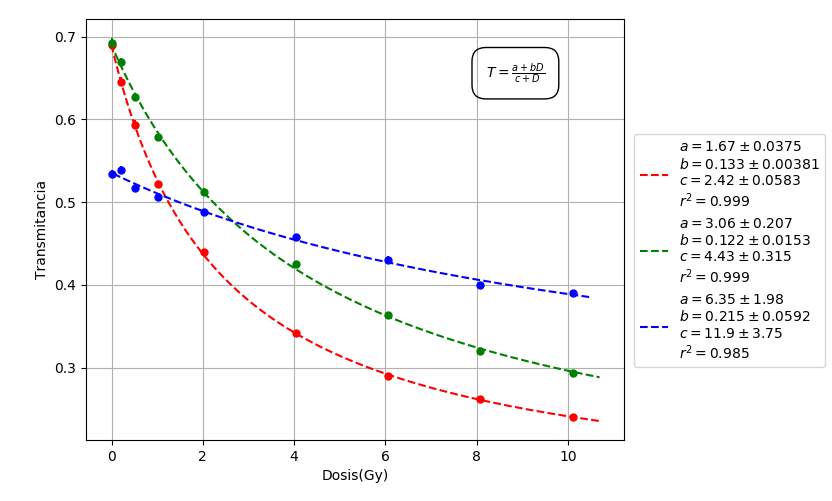
\includegraphics[width=0.7\linewidth]{images/calibracionMulti_2.png}
	\caption{Curva de calibración de 0 a 10 Gy}
\end{figure}
\end{frame}

\subsection{Efectos de otros parámetros}

\begin{frame}{Posición de la película}
\begin{figure}[htp]% [H] is so declass\'e!
	\centering
	\begin{minipage}{0.45\textwidth}
		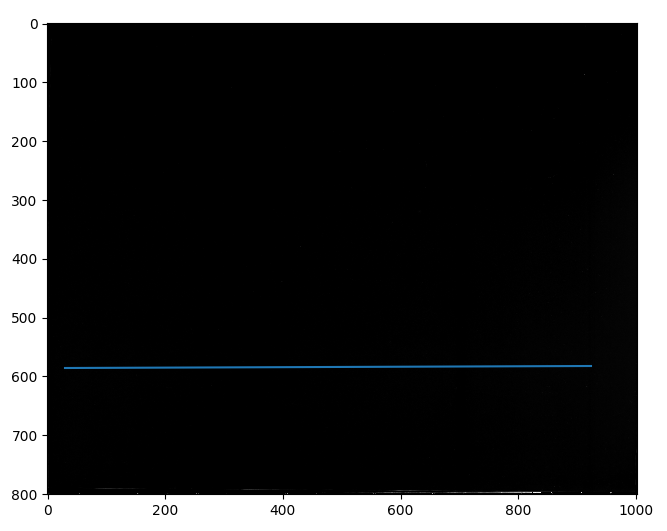
\includegraphics[width=\textwidth]{images/imagenPerfilMapaCeroHorizontal.png}
	\end{minipage}\hfill
	\begin{minipage}{0.45\textwidth}
		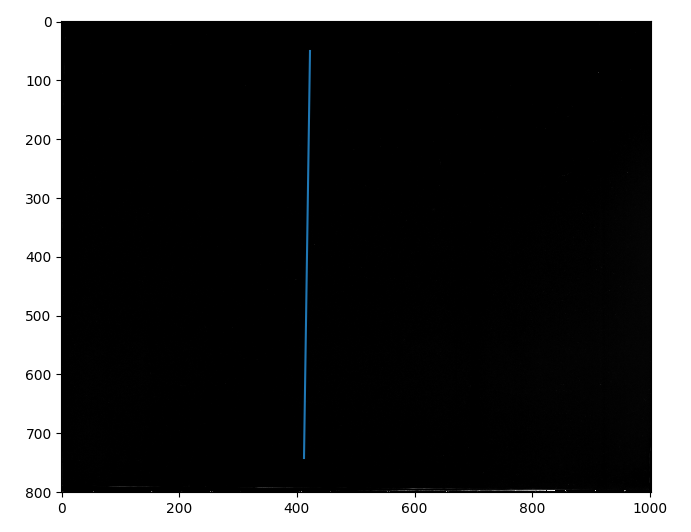
\includegraphics[width=\textwidth]{images/imagenPerfilMapaCeroVertical.png}
	\end{minipage}\par
	\begin{minipage}{0.45\textwidth}
		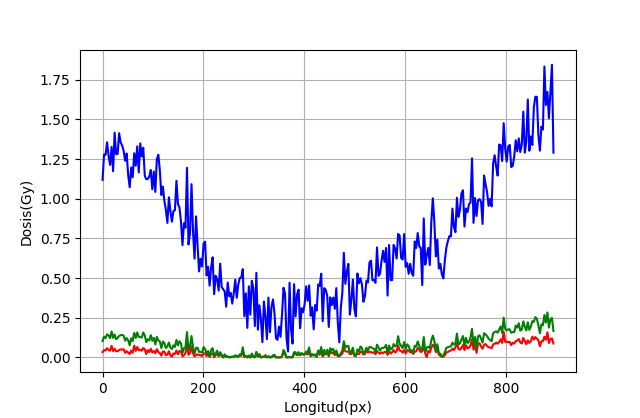
\includegraphics[width=\textwidth]{images/perfilDosisCeroHorizontal.png}
	\end{minipage}\hfill
	\begin{minipage}{0.45\textwidth}
		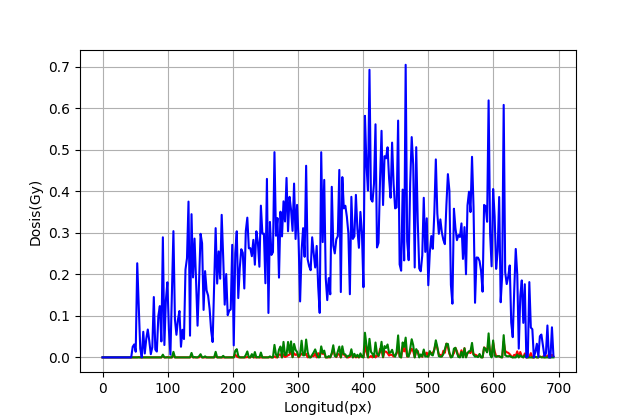
\includegraphics[width=\textwidth]{images/perfilDosisCeroVerticalEnCentro.png}
	\end{minipage}
	\caption{Perfiles de dosis}
\end{figure}
\end{frame}

\begin{frame}{Método multicanal}
\begin{figure}[htp]% [H] is so declass\'e!
	\centering
	\begin{minipage}{0.45\textwidth}
		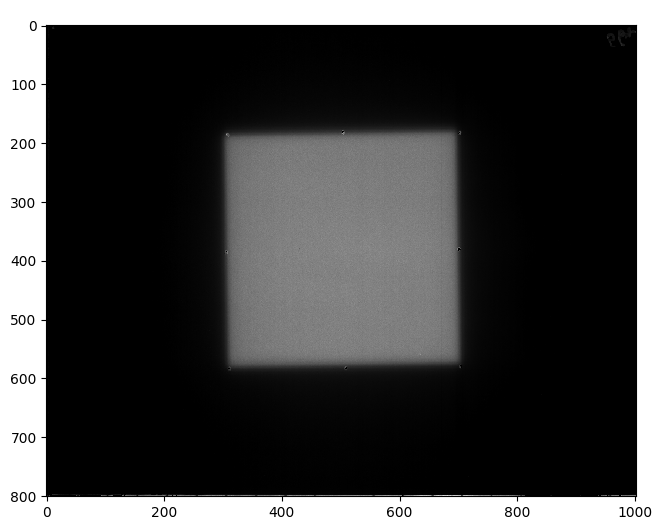
\includegraphics[width=\textwidth]{images/mapaCuadradoConMulticanal.png}
	\end{minipage}\hfill
	\begin{minipage}{0.6\textwidth}
		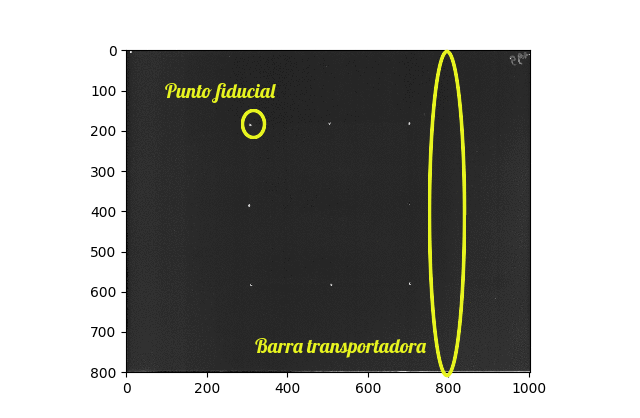
\includegraphics[width=\textwidth]{images/fondoCuadradoConLabel.png}
	\end{minipage}
	\caption{Mapa cuadrado con separación multicanal}
\end{figure}
\end{frame}

\begin{frame}{Método multicanal}
\begin{figure}[htp]% [H] is so declass\'e!
	\centering
	\begin{minipage}{0.6\textwidth}
		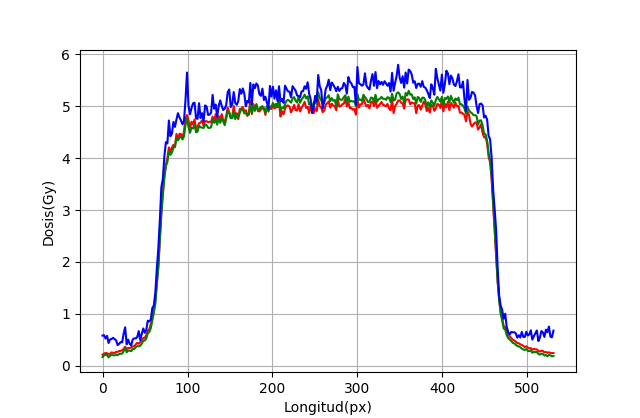
\includegraphics[width=\textwidth]{images/perfilDosisCuadradoUnoSolo.png}
	\end{minipage}\hfill
	\begin{minipage}{0.6\textwidth}
		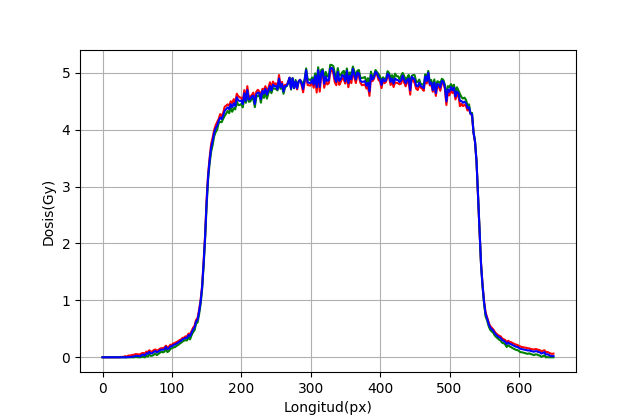
\includegraphics[width=\textwidth]{images/perfilDosisCuadradoMulticanal.png}
	\end{minipage}
	\caption{Perfiles de dosis para cuadrado de 5 Gy}
\end{figure}
\end{frame}

\subsection{Mapas de dosis}

\begin{frame}{Mapas de dosis}
\begin{figure}[htp]% [H] is so declass\'e!
	\centering
	\begin{minipage}{0.45\textwidth}
		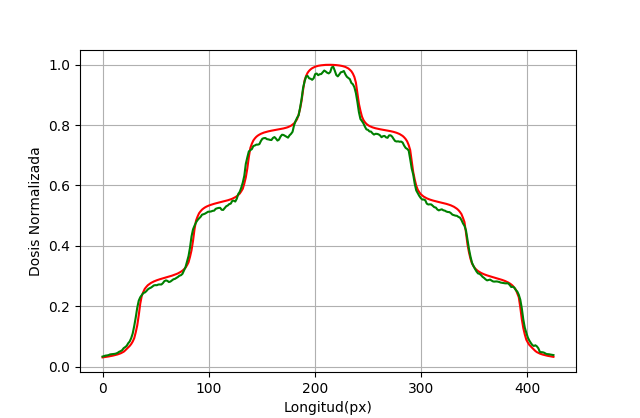
\includegraphics[width=\textwidth]{images/perfilPiramideNormalizado.png}
	\end{minipage}\hfill
	\begin{minipage}{0.45\textwidth}
		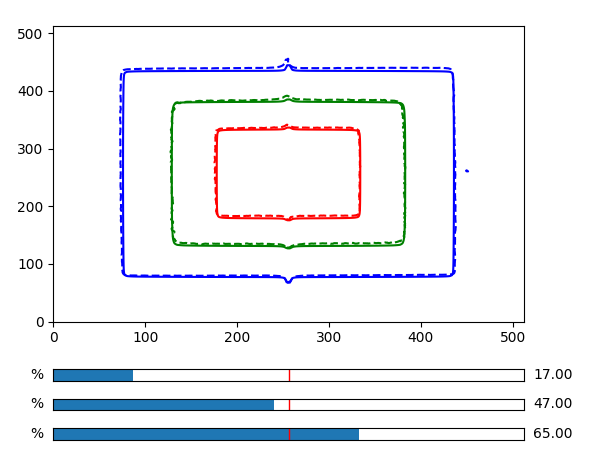
\includegraphics[width=\textwidth]{images/isodosisPiramide2.png}
	\end{minipage}\par
	\begin{minipage}{0.45\textwidth}
		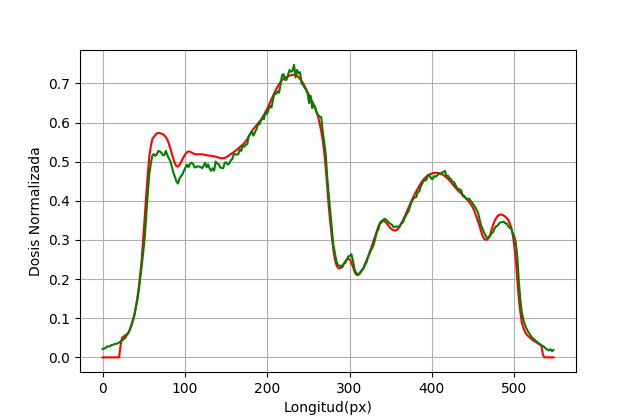
\includegraphics[width=\textwidth]{images/perfilDosisMama.png}
	\end{minipage}\hfill
	\begin{minipage}{0.45\textwidth}
		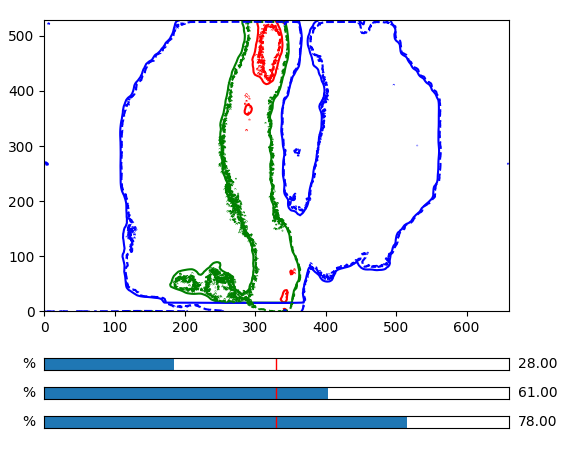
\includegraphics[width=\textwidth]{images/curvasIsodosisMama.png}
	\end{minipage}
	\caption{Análisis de mapas de dosis}
\end{figure}
\end{frame}

\subsection{Comparaciones a plan}

\begin{frame}{Comparaciones a plan}
\begin{figure}[htp]% [H] is so declass\'e!
	\centering
	\begin{minipage}{0.45\textwidth}
		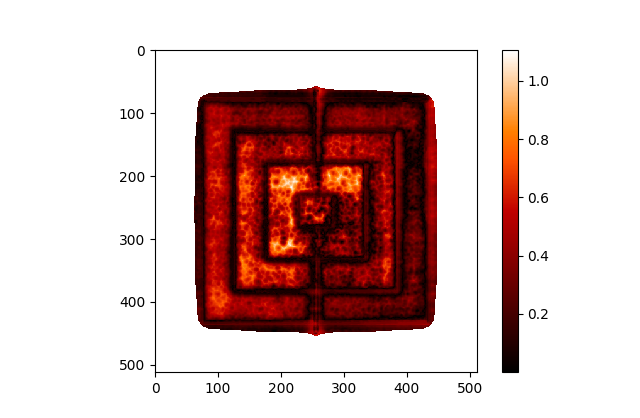
\includegraphics[width=\textwidth]{images/gammaPiramideCalor.png}
	\end{minipage}\hfill
	\begin{minipage}{0.45\textwidth}
		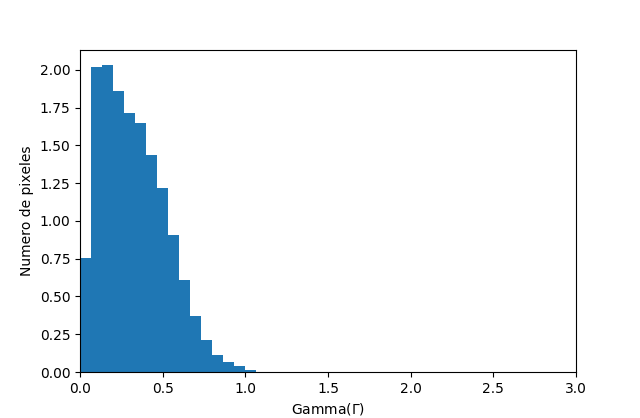
\includegraphics[width=\textwidth]{images/histogramaGammaPiramide.png}
	\end{minipage}\par
	\begin{minipage}{0.45\textwidth}
		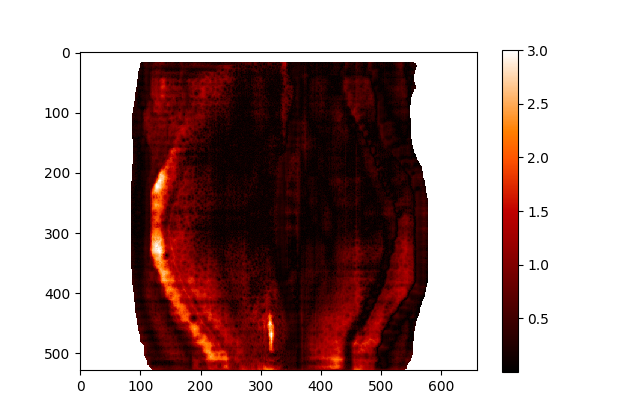
\includegraphics[width=\textwidth]{images/gammaMama.png}
	\end{minipage}\hfill
	\begin{minipage}{0.45\textwidth}
		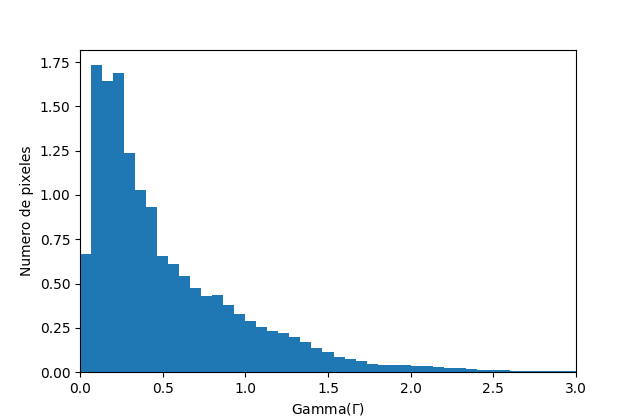
\includegraphics[width=\textwidth]{images/histogramaDosisMama.png}
	\end{minipage}
	\caption{Comparaciones $\Gamma$}
\end{figure}
\end{frame}

\section{Conclusiones}

\begin{frame}{Conclusiones}
	\begin{itemize}
		\item Las películas radiocrómicas son útiles para realizar aseguramiento de calidad en procesos de radioterapia.
		\item El procedimiento para usarlas es susceptible a varios parámetros que modifican las mediadas y deben ser controlados.
		\item Esto se puede realizar mediante el programa diseñado para este propósito.
	\end{itemize}
\end{frame}




\section{Bibliografía}
\begin{frame}[allowframebreaks]
\frametitle{Referencias}
\nocite{*}
\bibliographystyle{ieeetr}
\bibliography{references}
\end{frame}



\end{document}